\section*{Increasing the number of simultaneous
examples}

2018/07/10 - SYNALP - Esteban MARQUER

\subsection{Paradigm}

The test is run on a small number of epoch (20), with a minimal model
and a new training algorithm.

The training algorithm used is a \textbf{mini-batch training}, meaning
we compute the output for multiple examples all at once, we compute an
averaged loss over those examples, and we update the model.

The potential effects of this algorithm are:
\begin{itemize}
\item an increase of GPU memory usage, as computations are done on larger data;
\item a decrease of computation time, with the number of computations reduced;
\item a smother training loss, because it is averaged over multiple examples;
\item avoidance of some local minima.
\end{itemize}

A second test with random batch-size between 1 and 1000 was done on 50
epoch, to evaluate the effect of the batch size and find an optimum.

\subsection{Results}

\subsubsection{GPU memory usage}

As more examples are fed to the model, there is a very slight increase
in GPU memory usage: 0.013e7 B, corresponding to 127kiB (this amount is
negligible with more than 10GiB available and a current usage of about
10MiB).

\textbf{Conclusion:} increasing the number of simultaneous examples has
no substantial downsides memory-wise.

\begin{figure}[ht]
\centering
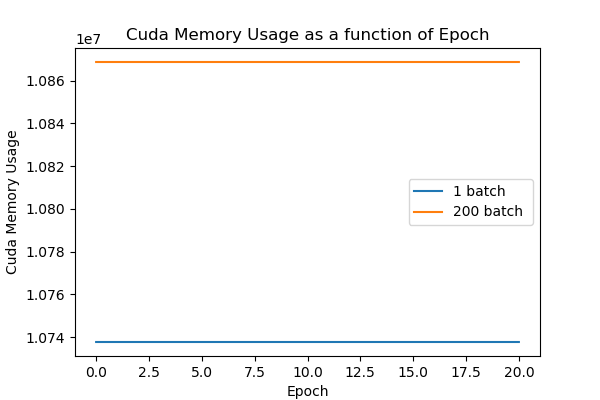
\includegraphics{parts/appendix/reports-papud/2018_07_11-Simultaneous_batches/memory.png}
\caption{memory usage}
\end{figure}

\subsubsection{Loss and accuracy}

As loss is averaged on multiple examples, it should be smoother. But,
probably because the number of simultaneous examples is too small, there
is no noticeable change of loss, with the curves superposed.

\textbf{Conclusion:} increasing the number of simultaneous examples has
no substantial effect loss-wise.

\begin{longtable}[]{@{}lll@{}}
\hline
Train. + Valid. & Training only & Validation only\tabularnewline
\hline
\endhead
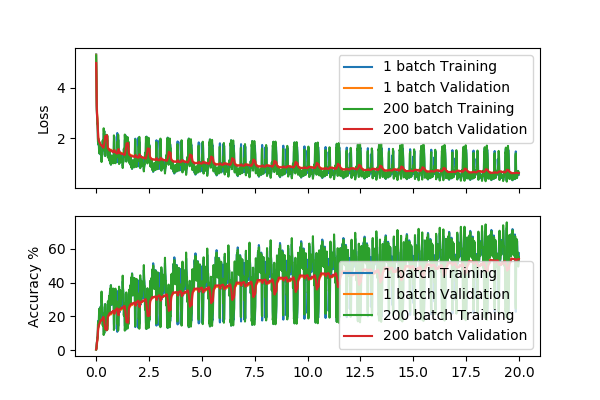
\includegraphics[width=.3\textwidth]{parts/appendix/reports-papud/2018_07_11-Simultaneous_batches/loss.png} & 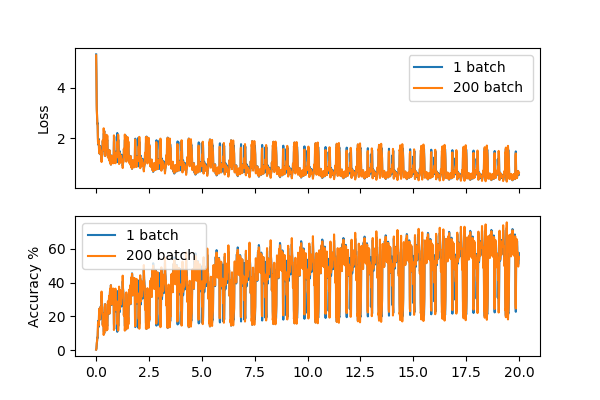
\includegraphics[width=.3\textwidth]{parts/appendix/reports-papud/2018_07_11-Simultaneous_batches/loss_train.png} &
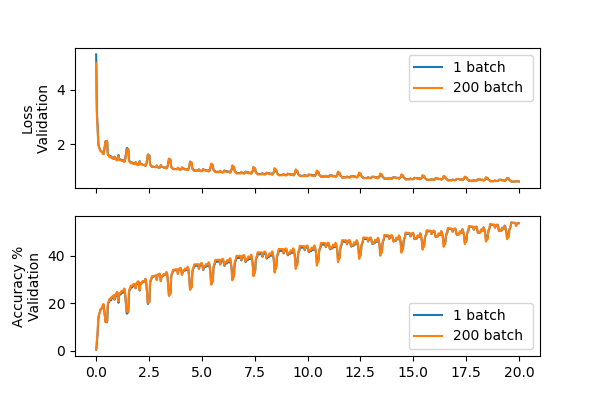
\includegraphics[width=.3\textwidth]{parts/appendix/reports-papud/2018_07_11-Simultaneous_batches/loss_valid.png}\tabularnewline
\hline
\end{longtable}

\subsubsection{Computation time}

The computations done on GPU benefit from grouping similar operations.
By computing multiple examples together, we can use this property to
speed up training. Moreover, retro-propagation and model updates are
less frequent, reducing computational load and training time.

The best-case time allow an improvement from 10ms to less than 2ms per
\textbf{training} sequence with a batch-size of 50, and the worst-case
one allow 4ms per training sequence with a batch-size of 200.

A small gain can be achieved on \textbf{validation} time by increasing
batch size over 50, but increasing it more has no effect.

\textbf{Conclusion:} increasing the number of simultaneous examples
leads to a notable improvement of computation time.

\begin{longtable}[]{@{}ll@{}}
\hline
Training time & Validation time\tabularnewline
\hline
\endhead
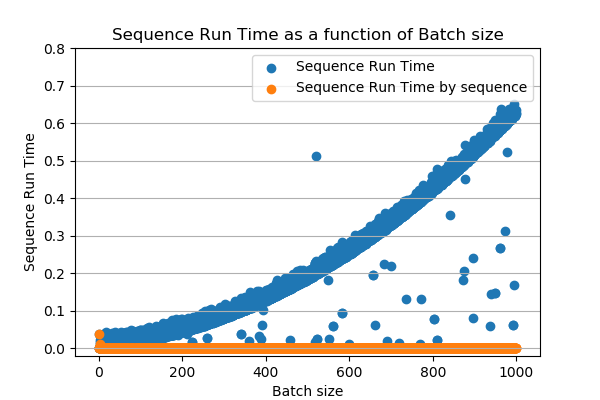
\includegraphics[width=.45\textwidth]{parts/appendix/reports-papud/2018_07_11-Simultaneous_batches/sequence_time.png} &
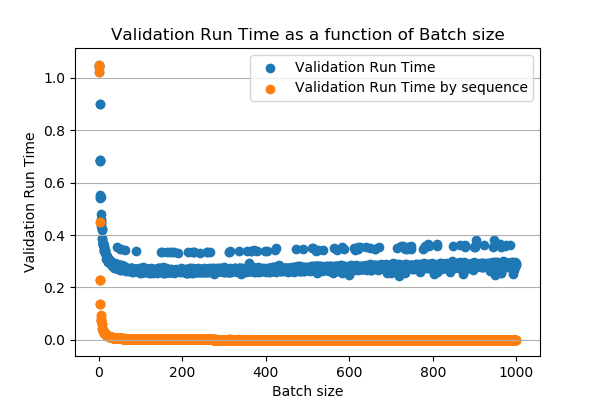
\includegraphics[width=.45\textwidth]{parts/appendix/reports-papud/2018_07_11-Simultaneous_batches/valid_time.png}\tabularnewline
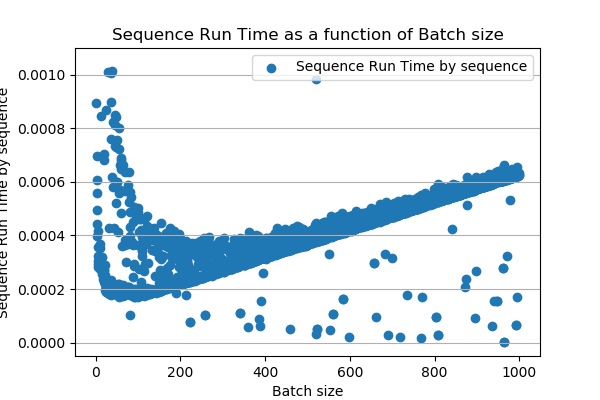
\includegraphics[width=.45\textwidth]{parts/appendix/reports-papud/2018_07_11-Simultaneous_batches/sequence_time_.png} &
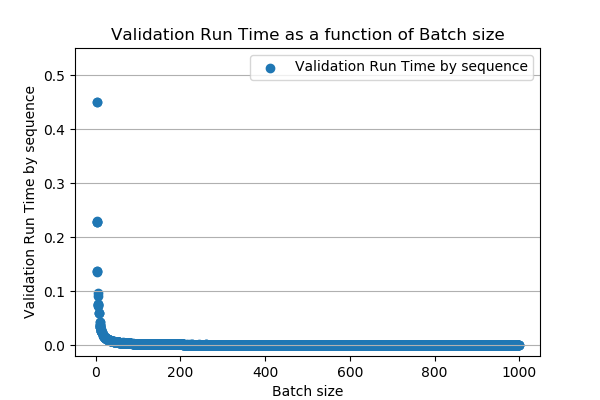
\includegraphics[width=.45\textwidth]{parts/appendix/reports-papud/2018_07_11-Simultaneous_batches/valid_time_.png}\tabularnewline
\hline
\end{longtable}

\subsection{Conclusion}

Even if there is no improvement of loss or memory, the gain in
computation time is enough to accept this algorithm.

The ideal batch-size (with the current node ``grele'') is between 50 and
200. In future works, a batch-size of 200 will be used, as it present
the best worst- and best-case time performances.

\subsection{Improvements and next
steps}

\subsubsection{Dynamic corpus}

The dynamic corpus implementation is ready (except small details) and
working, only integration is left.

\paragraph{Buffer size}

The dynamic corpus can use a buffer, and the size of this buffer must be
at least the size of the batch. It will be necessary to test which size
is optimal. An optimal buffer has the minimal size to make computation
time over the buffer size only slightly higher than pre-loading time. It
allows training to continue without interruption, while maintaining a
low memory usage.
